\section{Time plan}
% TODO(anton):
% - Decide on suitable iterations
% - Include GANTT Chart in a more readable format
%

A time plan has been devised to aid the project's scope being realistic in relation to the given time restrictions.
This includes time management of administrative tasks such as meetings, the developing of the end product as well as the final report.

\subsection{Meetings and work sessions}
All the group members have agreed to meet twice a week to mainly discuss the status of the project, distributing workload and to discuss further improvements or goals.
The internal meetings occur weekly every Monday and Thursday lunch from 12.10 to 13.00.
Also, on Tuesdays the group has reoccurring meetings with the project's supervisor for feedback, ideas, and to help guide the project in the right direction.
All group members are expected to attend all meetings and therefore follow an opt-out regimen.

Additionally, on Thursday afternoon and throughout Friday the group has decided to meet for common work sessions on a weekly basis.
The intended reason for these sessions is for the group to sit down together and help each other solve problems that often require communication between the different implementations.
Furthermore, the sessions make each member more approachable and keep group members updated on the overall status of the project.
These are not mandatory but still enforces an opt-out regimen to encourage more collaboration.

\subsection{Development of end product}
The three identified subproblems, described in section~\nameref{sec:problem}, facilitates a natural division of work since each of the subtasks can almost entirely be developed in isolation.
For instance the road generation can start off by only considering a strictly flat terrain.
Each subproblem is therefore further broken down into iterations so that the different systems can be developed simultaneously with as few dependency conflicts as possible.

Each iteration of a subproblem will start off as an isolated simple solution and increase in complexity and coupling with the other subsystems.
This approach will aid in working in a more cost-effective way when developing the end product.

Once all subtasks have undergone all iterations, our efforts will be targeted at fine-tuning the final solution as well as implementing as many of our stretch goals as possible.

\subsubsection{Landscape Generation}
\begin{description}
  \item[Iteration 1] Generate a simple height-map terrain mesh.
  \item[Iteration 2] Texture the terrain based on height levels.
  \item[Iteration 3] Populate the terrain with lakes, oceans and foliage.
\end{description}

\subsubsection{Road Generation}
\begin{description}
  % \item[iteration 0] Convert bezier curve into a road mesh. % this can be developed alongside iteration 1 so it doesn't fit my stupid model...
  \item[Iteration 1] Procedurally generate a convincing road-network on a 2D plane.
  \item[iteration 2] Convert the conceptual road-network into a road mesh.
  \item[Iteration 3] When generating a road from point A to point B, take the height difference in the underlying terrain into account in order to create a natural looking path.
\end{description}

\subsubsection{Building Generation}
\begin{description}
  \item[Iteration 1] Procedurally generate simple block buildings of skyscrapers and villas.
  \item[Iteration 2] Given a plot of land, populate it with suitably placed buildings.
\end{description}

\subsection{Final report}
When it comes to the final written report we are expected to continuously work on the final report during the development.
However we have also set a three week period strictly dedicated to finalizing the report.
At that point we expect the algorithm to be complete as to prioritize the final report.

\subsection{Project plan chart}
To get an overview of our time plan we have decided to include a GANTT chart seen in Figure~\ref{fig:time-plan} that roughly describe the expected time of the different tasks.

\newpage
\begin{figure}[H]
  \centering
  \vspace*{-1.0cm}
  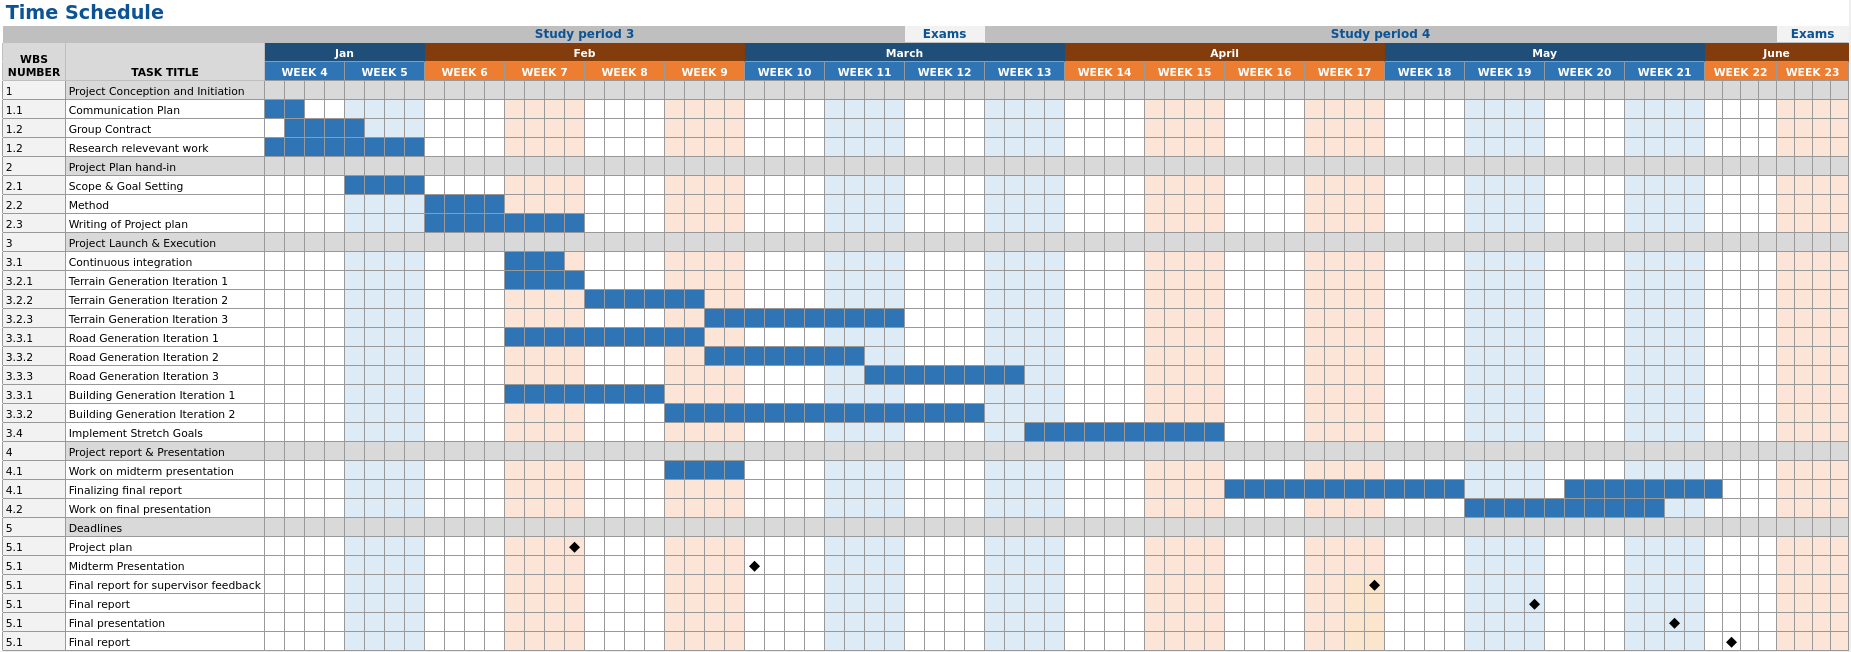
\includegraphics[angle=90, width=0.5\textwidth]{figure/time-plan.png}
  \caption{Time plan}
  \label{fig:time-plan}
\end{figure}

